\documentclass[conference]{IEEEtran}

\usepackage{amsmath, amssymb}
\usepackage{graphicx}
\usepackage{array}
\usepackage{multirow}
\usepackage{hyperref}

% for better table formatting
\newcommand{\tabincell}[2]{\begin{tabular}[c]{@{}#1@{}}#2\end{tabular}}

\begin{document}

\title{Unsupervised Learning Technique for Binarization of Gray Scale Text Images}

\author{
    \IEEEauthorblockN{Saumya Srivastava}
    \IEEEauthorblockA{Dept. Human Computer Interaction\\
    Indian Institute of Information Technology Allahabad, India\\
    saumyasrivastava22@gmail.com}
    \and
    \IEEEauthorblockN{Prof. Sudip Sanyal}
    \IEEEauthorblockA{Dept. Intelligent Systems\\
    Indian Institute of Information Technology Allahabad, India\\
    ssanyal@iiita.ac.in}
}

\maketitle

\begin{abstract}
This paper suggests an unsupervised learning technique for binarization of gray scale text images based on fusion of existing approaches. The existing binarization approaches have though resolved issues of degraded contrast, varied intensity, shadow, smudges, bleed through and smear to a certain extent, yet none of the existing algorithms are capable to work out all the issues independently. However, these have also led to issues like broken characters and merged characters. Some of the standard algorithms in this field have been chosen as the core methods to produce partial binarization results. The decision on these partial binarized results has been fused using three different proposed approaches. The benchmark of performance evaluation are those set by DIBCO. The standard dataset along with the ground truth have also been taken from the same. Our binarized results produced from the above methods have given better results in contrast to DIBCO-2011 and have also surpassed the failure cases of DIBCO 2011. The Results and Analysis section comprehends the conclusion drawn.
\end{abstract}

\begin{IEEEkeywords}
Unsupervised Learning, Broken Characters, Merged Characters, Binarization
\end{IEEEkeywords}

\section{INTRODUCTION}
The era of retrievable information has come. Various documents need to be digitized for its users for quicker, faster and cheaper access and this requires Optical Character Recognition, particularly for ancient artifacts. Since ancient artifacts follow different textual language, characters, fonts and varying size thus trained OCRs like ABBYY FineReader fail to digitize them without manual supervision and script experts.

Binarization marks the commencement of the character recognition pipeline. Minor error at this stage leads to cumulative misclassification at a later stage ultimately hampering the recognition results. A brief study of previously proposed and applied methodologies leads to the inference that in spite of major advances in this field, the results are not close to the ground truth. Several binarization algorithms (with associated frameworks), together with required preprocessing, have resolved issues of degraded contrast, varied intensity, shadow, smudges, bleed through and smear to a certain extent. However, these have also led to newly created issues like damaged and broken characters and merged characters. This is the outcome of over or under binarization that happens with several approaches.

A brief description of a few surveyed approaches has been given in the next section along with their respective pros and cons. The inference drawn is that the misclassified pixels are a result of close proximity with the global or local threshold (whichever is applicable) in all methods. Interestingly, it has been observed that a set of pixels which get misclassified by one method may be correctly classified by another method. This leads to the possibility of exploring techniques that combine the results of all the techniques using voting and/or some measure of confidence. Thus, we introduce a parameter, based on the closeness of the pixel to the threshold, to decide the confidence of the pixel to belong to a certain class. Confidence has been mathematically defined as the absolute distance of the pixel value from its corresponding threshold divided by the corresponding threshold. This acts as the prime constituent of the proposed frameworks.

This paper presents three approaches, each sharing the same baseline but building the resultant binarized image in a different manner. The key objective of all the three approaches is to promote the existence of valid pixel and demote the existence of misclassified pixels in the resultant binarized image.

Our experiments have been performed using the standard evaluation parameters setup by DIBCO. In addition, tabular comparison has also been made w.r.t. to DIBCO 2011 results and US Patent sharing a similar perspective regarding Confidence Value. Sections below discuss in detail the applied methodology and experimental results along with its evaluated value w.r.t. the ground truth. This section is followed by the literature survey section, briefly discussing the studied approaches and why they inspire the present approach, also discussing similar methods on confidence value in brief. Thereafter the three algorithmic approaches have been discussed in detail along with their experimental results.

\section{RELATED WORK}

\subsection{Ostu's Method with Framework}
Amongst all, Ostu's \cite{otsu1979threshold} method has been one of the earliest algorithms. An additional Framework \cite{chi2012learning} has been applied to remove the drawbacks of the original method. The major drawback of this framework is that pixels in close proximity to the foreground pixels tend to get misclassified, thereby affecting its performance by a significant amount.

\subsection{Niblack's Method}
Niblack's algorithm \cite{niblack1986introduction} calculates a local, neighborhood dependent, threshold for each pixel in the image. This requires $m$ which is the local mean of all the pixels in the rectangular window and $s$, the local standard deviation within the window.
\begin{equation}
T_{\text{Niblack}} = m + k\sqrt{\frac{1}{N}\sum(p_i - m)^2}
\end{equation}
In the above, $N$ is the number of pixels in the local window, $m$ is the average of all the pixel values $p_i$ and $k$ is defined as Niblack's factor with a default value set at $-0.2$. This method improves binarization by accurately identifying the foreground but fails to avoid noise in the background.

\subsection{Sauvola's Method}
Sauvola's algorithm \cite{sauvola1997adaptive} improves the Niblack's algorithm by calculating the threshold based on the dynamic range of image's gray value standard deviation, $R$ given by the following equation.
\begin{equation}
T_{\text{Sauvola}} = m\left(1 - k\left(1 - \frac{S}{R}\right)\right)
\end{equation}
where $k$ and $R$ are constants with values $0.5$ and $128$ respectively. This method performs well when performance is measured in terms of F- Measure but certainly degrades when it comes to recognition of images in which there is little difference in gray level value of the foreground and background. This has been shown in the next section.

\subsection{Wolf's Method}
Wolf et al. \cite{wolf2003extraction} proposed this algorithm to resolve the above mentioned issue by normalizing the mean value and averaging the contrast in the local window to compute the threshold as:
\begin{equation}
T_{\text{Wolf}} = (1 - k)m + kM + k(m - M)\frac{S}{R}
\end{equation}
With $k = 0.5$, $M$ as the minimum gray level value of the entire image and $R$ as the maximum gray level standard deviation among all the local neighborhoods of the considered window. Since the values of $M$ and $R$ are global in nature, thus for uneven background this algorithm does not hold. Moreover, since backgrounds of historical documents tend to have this issue, thus this algorithm cannot serve its purpose in this scenario.

\subsection{Feng's Method}
This method \cite{feng2004contrast} eradicates the issues in the above approach by calculating $R$ in the local secondary window. Mean $m$, standard deviation $s$ and the minimum of gray level values in the window are calculated for the primary window lying within the secondary window. The threshold is calculated as:
\begin{equation}
T_{\text{Feng}} = (1 - \alpha_1) m + \alpha_2 \left(\frac{S}{R}\right)(m - M) + \alpha_3 M
\end{equation}
where constants $\alpha_2 = k_1 + (s/R)^\gamma$ and $\alpha_3 = k_2 + (s/R)^\gamma$. The constants $\gamma$, $\alpha_1$, $k_1$ and $k_2$ take experimentally determined values of $2$, $0.1-0.2$, $0.15-0.25$ and $0.01-0.05$ respectively. This algorithm tends to outperform all other algorithms provided the size of the secondary window is that of the size of a character.

\subsection{NICK's Method}
This method \cite{khurshid2009comparison} is a similar in flavor to Niblack's algorithm except that it improves binarization by minimizing the noise in the background which Niblack's method fails to achieve. The threshold is given as:
\begin{equation}
T_{\text{NICK}} = m + \sqrt{\frac{1}{N}\sum p_i^2 - m^2}
\end{equation}
where $N$ is the number of pixels in the local window.

A US Patent (Patent No. - US 6411737 B2)\cite{uspatent} uses a similar concept, but of aggregate Confidence value of every Binarization Algorithm applied on the input measure as a means to decide which algorithm for a scanned image gives the best result. Tabular comparison with this perspective has also been statistically analyzed.

\section{PROPOSED APPROACHES}
We propose three unsupervised statistical frameworks using some of the algorithms discussed above. The resultant binarized image of the above approaches and the corresponding normalized confidence matrix contribute to the decision for each pixel in the image and this acts as a feature towards the end result.

In the first approach, i.e. Voting Algorithm, all algorithms cast their votes in favor of either foreground or background. Majority of the same decides the final pixel value in the resultant image. For example, let us consider a gray scale image. A total of five binarized images will be produced by five different algorithms described in the earlier section. If, for the pixel at position (i, j), two algorithms cast votes in favor of foreground and the remaining three cast vote in favor of background then, background having majority takes lead in the resultant image. This is repeated for all the pixels in the image. Note: Since the average performance of Wolf's Method \cite{wolf2003extraction} was too low, thus it has been struck off this experiment.

In the second approach, i.e. Weighted Voting Algorithm, for a pixel in Image I, all algorithms favoring foreground add its confidence value to the foreground vote for the respective pixel and those favoring background add its confidence value to the background vote. Majority in the value of either of the vote decides its class in the resultant image. In the present work, the confidence of a particular algorithm for a given pixel is the ratio of distance of the pixel value from the threshold to the actual threshold value.

In the third and last proposed approach, i.e. the Maximum Confidence Algorithm, the maximum of all the confidence values of all the included algorithms for a pixel $I(i,j)$ and its corresponding value in its binary image i.e. foreground or background decides its pixel value in the resultant image. For example, if the second algorithm has the maximum confidence value for $I(i,j)$ then the discrete value (foreground/background) in binarized image of Algorithm 2 is the value of $(i,j)$ in the resultant binarized image.

\section{EXPERIMENTAL RESULTS}
The experiments have been performed on the data set from DIBCO-2011\cite{dibco2011dataset}. Experimental Results of all the applied algorithms and the three proposed approaches in terms of F- Measure has been stated in the table below. Figure 1 gives a pictorial view of the same. Further, the actual recognition rate concludes the overall efficacy of the proposed approaches. The OCR used is ABBYY Fine Reader12 \cite{abbyy}.

From the Table 1, Sauvola's Method can be concluded as the best algorithm for binarization followed by the proposed Voted Algorithm which gives a comparable result. The Wolf's method results low thus has been sidelined in the proposed approaches. While the Weighted Vote approach gives a slightly lower F- measure, it has been experimentally concluded as the best approach on the basis of recognition rate in Table 4. An Inference has also been drawn that binarization results can't be judged on the basis of F- Measure alone. However, better PSNR value justifies improvement in performance w.r.t other base algorithms.

Table 2 shows that in spite of giving spectacular F- Measure, how Sauvola's PSNR falls, clearly indicating its failure to attain a good recognition in the long run. Table 2 at the same time also marks a good performance of Weighted Vote Confidence over simple voting algorithm. This has clearly justified in terms of Recognition Rate in Table 4. In addition to stated measures, Execution Time is marked as a considerable measure for performance. Since Binarization is an offline process and the overhead of the proposed algorithms is negligible over existing algorithms, thus quality of binarization is given more preference over time.

\begin{table}[!t]
\caption{COMPARISON OF ALL ALGORITHMS IN TERMS OF F-MEASURE}
\centering
\begin{tabular}{|l|c|c|c|c|c|c|c|c|c|}
\hline
Image & Otsu & Niblack & Sauvola & Wolf & Feng & NICK & Voted & Wt. Vote & Max. Conf. \\
\hline
PN1.png & 89.49 & 95.19 & 98.71 & 84.77 & 95.76 & 97.28 & 96.06 & 96.25 & 94.66 \\
PN2.png & 89.80 & 96.06 & 97.84 & 87.59 & 94.74 & 97.44 & 96.11 & 96.35 & 94.91 \\
PN3.png & 94.10 & 96.59 & 98.59 & 89.81 & 96.37 & 97.14 & 97.10 & 97.84 & 97.26 \\
PN4.png & 90.15 & 96.68 & 99.16 & 84.46 & 96.86 & 98.13 & 97.29 & 98.05 & 96.39 \\
PN5.png & 92.56 & 97.04 & 98.75 & 88.37 & 96.13 & 97.67 & 97.57 & 97.71 & 96.35 \\
PN6.png & 77.97 & 93.23 & 98.91 & 79.54 & 88.89 & 99.13 & 90.30 & 89.48 & 85.68 \\
PN7.png & 74.23 & 96.71 & 90.75 & 74.83 & 91.4 & 99.28 & 93.29 & 97.25 & 95.94 \\
PN8.png & 95.59 & 97.88 & 97.88 & 85.70 & 96.48 & 96.42 & 98.15 & 98.16 & 97.69 \\
\hline
\end{tabular}
\label{tab:fmeasure}
\end{table}

\begin{table}[!t]
\caption{COMPARISON OF ALL ALGORITHMS IN TERMS OF PSNR}
\centering
\begin{tabular}{|l|c|c|c|c|c|c|c|c|c|}
\hline
Image & Otsu & Niblack & Sauvola & Wolf & Feng & NICK & Voted & Wt. Vote & Max. Conf. \\
\hline
PN1.png & 0.8265 & 0.8318 & 0.8341 & 0.8299 & 83.21 & 0.8342 & 11.1996 & 11.4985 & 0.8104 \\
PN2.png & 0.5678 & 0.5728 & 0.5738 & 0.5675 & 0.5755 & 0.5747 & 11.2522 & 11.5207 & 0.5714 \\
PN3.png & 0.9144 & 0.9175 & 0.9158 & 91.28 & 0.9199 & 0.9190 & 12.4648 & 13.7472 & 0.9173 \\
PN4.png & 0.5487 & 0.5530 & 0.5555 & 0.5473 & 0.5940 & 0.5556 & 12.7774 & 14.1751 & 0.5530 \\
PN5.png & 0.6736 & 0.6776 & 0.6787 & 0.6722 & 0.6784 & 0.6790 & 13.2398 & 13.6833 & 0.6765 \\
PN6.png & 0.2416 & 0.2597 & 0.2543 & 0.2433 & 0.2487 & 0.2548 & 7.5289 & 7.2851 & 0.2400 \\
PN7.png & 0.1284 & 0.1407 & 0.1427 & 0.1289 & 0.1375 & 0.1428 & 9.0072 & 12.7070 & 0.1401 \\
PN8.png & 0.6743 & 0.6770 & 0.6773 & 0.6689 & 67.51 & 0.6774 & 14.3866 & 14.4267 & 0.6767 \\
\hline
\end{tabular}
\label{tab:psnr}
\end{table}

\begin{table}[!t]
\caption{COMPARISON OF ALL ALGORITHMS IN TERMS OF TIME (SECS)}
\centering
\begin{tabular}{|l|c|c|c|c|c|c|c|c|c|}
\hline
Image & Otsu & Niblack & Sauvola & Wolf & Feng & NICK & Voted & Wt. Vote & Max. Conf. \\
\hline
PN1.png & 1.17 & 0.77 & 0.56 & 1.08 & 0.67 & 0.39 & 0.06 & 0.27 & 0.19 \\
PN2.png & 0.46 & 0.51 & 0.51 & 0.61 & 0.54 & 0.28 & 0.04 & 0.17 & 0.10 \\
PN3.png & 0.45 & 0.49 & 0.49 & 0.59 & 0.44 & 0.21 & 0.04 & 0.16 & 0.09 \\
PN4.png & 1.33 & 1.46 & 1.21 & 1.67 & 1.59 & 0.64 & 0.21 & 0.81 & 0.73 \\
PN5.png & 0.48 & 0.55 & 0.44 & 0.57 & 0.42 & 0.23 & 0.04 & 0.09 & 0.10 \\
PN6.png & 1.28 & 1.43 & 1.27 & 1.64 & 1.48 & 0.64 & 0.13 & 0.55 & 0.53 \\
PN7.png & 0.37 & 0.41 & 0.36 & 0.46 & 0.37 & 0.16 & 0.03 & 0.05 & 0.06 \\
PN8.png & 0.32 & 0.32 & 0.31 & 0.36 & 0.33 & 0.14 & 0.02 & 0.06 & 0.06 \\
\hline
\end{tabular}
\label{tab:time}
\end{table}

Given below are images obtained from the above mentioned algorithms and our proposed approaches. The results shown below are for "image8.png" of DIBCO 2011 Dataset. This is followed by Table 4 which gives the Recognition Rate of each image using Sauvola's algorithm and all the proposed approaches. This is the measure that ultimately speaks how well binarization has been performed. The entries in Table 4 can be interpreted as follows: Considering the row for Image 3, the original image has 212 characters; however its ground truth correctly recognizes only 207 characters. Binarization using Sauvola's method has lead to the discovery of 198 correctly recognized characters while the weighted vote method gives a count of 207 characters.

\begin{table}[!t]
\caption{RECOGNITION RATE FOR ALL THE THREE PROPOSED APPROACHES AND SAUVOLA'S ALGORITHM (*Gt: Ground Truth. Blank Spaces Indicate Failure In Recognition.)}
\centering
\begin{tabular}{|l|c|c|c|c|c|}
\hline
DIBCO 2011 & Original & Sauvola & Voted & Weighted & Maximum \\
Image      &          & Image   & Image & Vote    & Confidence \\
\hline
Image 1 & 78 & - & - & GT-40 & - \\
Image 2 & 222 & - & 78 & 87 & 69 \\
        &     &   &    & GT-139 & \\
Image 3 & 212 & 198 & 179 & 287 & 195 \\
        &     &     &     & GT-207 & \\
Image 4 & 182 & 159 & 123 & 161 & 192 \\
        &     &     &     & GT-165 & \\
Image 5 & 252 & 117 & 102 & 112 & 99 \\
        &     &     &     & GT-144 & \\
Image 6 & 76 & - & - & 40 & 57 \\
        &    &   &   & GT-76 & \\
Image 7 & 39 & 31 & 30 & 35 & 24 \\
        &    &    &    & GT-39 & \\
Image 8 & 190 & 133 & 167 & 196 & 187 \\
        &     &     &     & GT-190 & \\
\hline
\end{tabular}
\label{tab:recognition}
\end{table}

It has been observed that in almost all images the Weighted Confidence Vote method gives enhanced results above other base methods. Thus, even though the F- measure seems to indicate that the Sauvola's method is the best, character recognition with the Weighted Confidence Vote approach appears to be the best.

Observations in Table 4 can be better understood on the examination of the images in Figure 1. We observe that Sauvola's method efficiently removes noise, but fails when intensity of pixel between the two classes is low, thus allowing misclassification. This phenomenon can be observed along the left margin of Figure 1(c). It becomes quite obvious for the confidence of Sauvola's method to be low for pixels close to threshold, but it is quite possible that other methods may produce a higher confidence value for these pixels and ultimately lead to correct classification. In such cases, the weighted confidence voting method gives weight- age to the result of such methods in terms of confidence above those leading to misclassification. This can be observed in Figure 1(h) in which we can see that some patches (along the left margin) have been recovered.

\begin{figure}[!t]
\centering
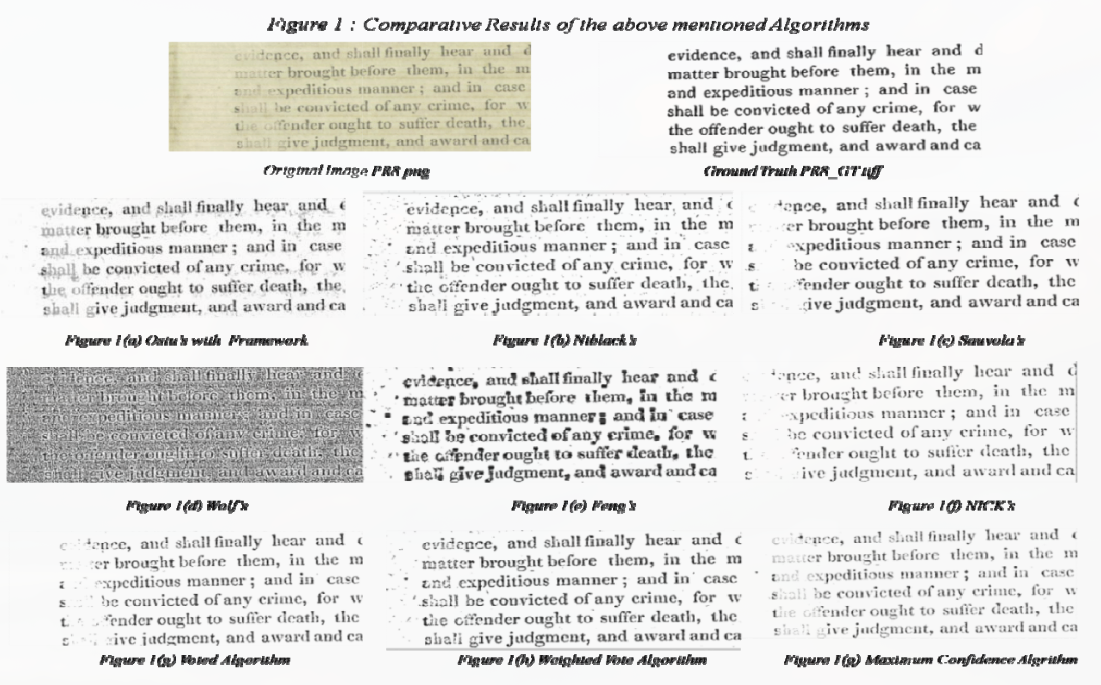
\includegraphics[width=0.9\columnwidth]{figure1.png}
\caption{Comparative Results of the above mentioned Algorithms. (a) Cuts to with Prunework, (b) Word Algorith, (c) Sauvola, (d) Wolf, (e) Feng, (f) NICK, (g) Voted, (h) Weighted Vote. (Actual images not reproduced.)}
\label{fig:results}
\end{figure}

\begin{table*}[!t]
\caption{COMPARISON OF PROPOSED RESULTS AGAINST WINNING ALGORITHMS OF DIBCO 2011 \cite{dibco2011results}}
\centering
\footnotesize
\begin{tabular}{|c|c|c|c|c|c|c|c|c|c|}
\hline
\multirow{2}{*}{DIBCO 2011} & \multicolumn{3}{c|}{PROPOSED METHODOLOGY} & \multicolumn{3}{c|}{RESULTS FROM CONTEST} \\
\cline{2-8}
 & Voted & Wt. Conf. & Max. Conf. & (10) & (08) & (11) \\
\hline
PR1.png & F-MEASURE & 96.06 & 96.25 & 94.66 & 94.90 & 92.90 & 94.2 \\
 & PSNR & 11.1996 & 11.4083 & 0.8304 & 17.8 & 16.4 & 17.2 \\
\hline
PR2.png & F-MEASURE & 96.11 & 96.35 & 94.91 & 77.2 & 82.8 & 70.3 \\
 & PSNR & 11.2522 & 11.5207 & 0.5714 & 11.9 & 13.2 & 10.2 \\
\hline
PR3.png & F-MEASURE & 97.10 & 97.84 & 97.26 & 94.80 & 93.80 & 96.5 \\
 & PSNR & 12.4848 & 13.7472 & 0.9173 & 17.3 & 16.5 & 18.9 \\
\hline
PR4.png & F-MEASURE & 97.29 & 98.05 & 96.39 & 95.8 & 92.8 & 94.8 \\
 & PSNR & 12.7774 & 14.1731 & 0.5530 & 19.6 & 17.7 & 19.5 \\
\hline
PR5.png & F-MEASURE & 97.57 & 97.71 & 96.35 & 93.3 & 92.7 & 94.8 \\
 & PSNR & 13.2390 & 13.4833 & 0.6765 & 16.7 & 17.1 & 18.5 \\
\hline
PR6.png & F-MEASURE & 90.30 & 89.48 & 85.68 & 89.9 & 92.6 & 84.9 \\
 & PSNR & 7.5230 & 7.2051 & 0.2460 & 0.62 & 1.4 & 17.9 \\
\hline
PR7.png & F-MEASURE & 93.29 & 97.25 & 95.94 & 44.6 & 21.1 & 79.1 \\
 & PSNR & 9.0072 & 12.7070 & 0.1401 & 10.2 & 7.6 & 19.2 \\
\hline
PR8.png & F-MEASURE & 98.15 & 98.16 & 97.69 & 86.10 & 86.2 & 88.5 \\
 & PSNR & 14.3866 & 14.4267 & 0.6767 & 14.6 & 14.6 & 15.3 \\
\hline
AVERAGE & F-MEASURE & 95.74 & 96.39 & 94.86 & 69.35 & 81.66 & 87.88 \\
 & PSNR & 11.48 & 12.33 & 0.5712 & 12.33 & 15.56 & 17.68 \\
\hline
\end{tabular}
\label{tab:dibco2011}
\end{table*}

Table 5 statistically compares the performance of winning algorithms of DIBCO 2011\cite{gatos2011icdar} with the proposed frameworks. It also represents the result of another experiment performed on the binarized results of DIBCO 2011\cite{dibco2011results} algorithms. The experiment has successfully achieved of the target of overcoming the failure cases of winning algorithms of DIBCO 2011 without compromising with the result of other images. Table 6 compares the result of idea of using confidence value in \cite{uspatent} against those proposed in this paper.

It is pertinent to point out at this stage that the results are also affected by the specific OCR used for the character segmentation and recognition. This is demonstrated in a comparison between the results obtained using ABBYY Fine Reader and Tesseract.

\begin{table*}[!t]
\caption{COMPARISON OF PROPOSED RESULTS AGAINST IDEA OF US PATENT CONFIDENCE VALUE \cite{uspatent}}
\centering
\footnotesize
\begin{tabular}{|c|c|c|c|c|c|c|c|c|}
\hline
\multirow{2}{*}{Image No.} & \multicolumn{2}{c|}{Voted Framework} & \multicolumn{2}{c|}{Weighted Voting Framework} & \multicolumn{2}{c|}{Maximum Confidence} & \multicolumn{2}{c|}{US Patent} \\
\cline{2-9}
 & FM & PSNR & FM & PSNR & FM & PSNR & FM & PSNR \\
\hline
PR1.png & 96.06 & 11.29 & 96.25 & 11.41 & 94.66 & 0.83 & 89.49 & 0.83 \\
PR2.png & 96.11 & 11.25 & 96.35 & 11.53 & 94.91 & 0.57 & 89.8 & 0.57 \\
PR3.png & 97.10 & 12.59 & 97.84 & 13.74 & 97.26 & 0.92 & 94.1 & 0.91 \\
PR4.png & 97.29 & 12.78 & 98.05 & 14.71 & 96.39 & 0.55 & 90.15 & 0.55 \\
PR5.png & 97.57 & 13.24 & 97.71 & 13.48 & 96.35 & 0.68 & 92.56 & 0.67 \\
PR6.png & 90.30 & 7.52 & 89.48 & 7.20 & 85.68 & 0.25 & 77.07 & 0.24 \\
PR7.png & 93.29 & 9.01 & 97.25 & 12.71 & 95.94 & 0.14 & 99.75 & 0.14 \\
PR8.png & 98.15 & 14.38 & 98.16 & 14.43 & 97.69 & 0.68 & 97.85 & 0.67 \\
\hline
\end{tabular}
\label{tab:uspatent}
\end{table*}

\section{CONCLUSION}
Three approaches have been proposed for an unsupervised fusion of the decisions of various binarization algorithms such that the benefits of one algorithm is able to overcome the drawbacks of other algorithm. It is found that while Sauvola's method gives the best result if F- measure is used, the actual recognition rate increases when we use fusion with a weighted voting. The weight given to a the decision of a particular algorithm depends on the confidence of that algorithm for a given pixel.

Over- binarized results have also been taken into consideration to provide more weight to the broken character pixels, the unnecessary background noise is filtered out with the help of other existing algorithms. Thus the conclusion drawn from the above experiment is that though the proposed Voted Algorithm has though given a comparable F- Measure w.r.t Sauvola's Binarization Method followed by Weighted Vote Algorithm, but Weighted Vote Algorithm gives a better average recognition rate in comparison to the rest of the algorithms discussed above (inclusive of algorithms given previously).

But the algorithms fail to binarize in low contrast images, i.e. when the difference between the foreground and background is less. A simple contrast stretching preprocessing experiment was also performed to resolve the issue but no significant change was observed.

\begin{figure}[!t]
\centering
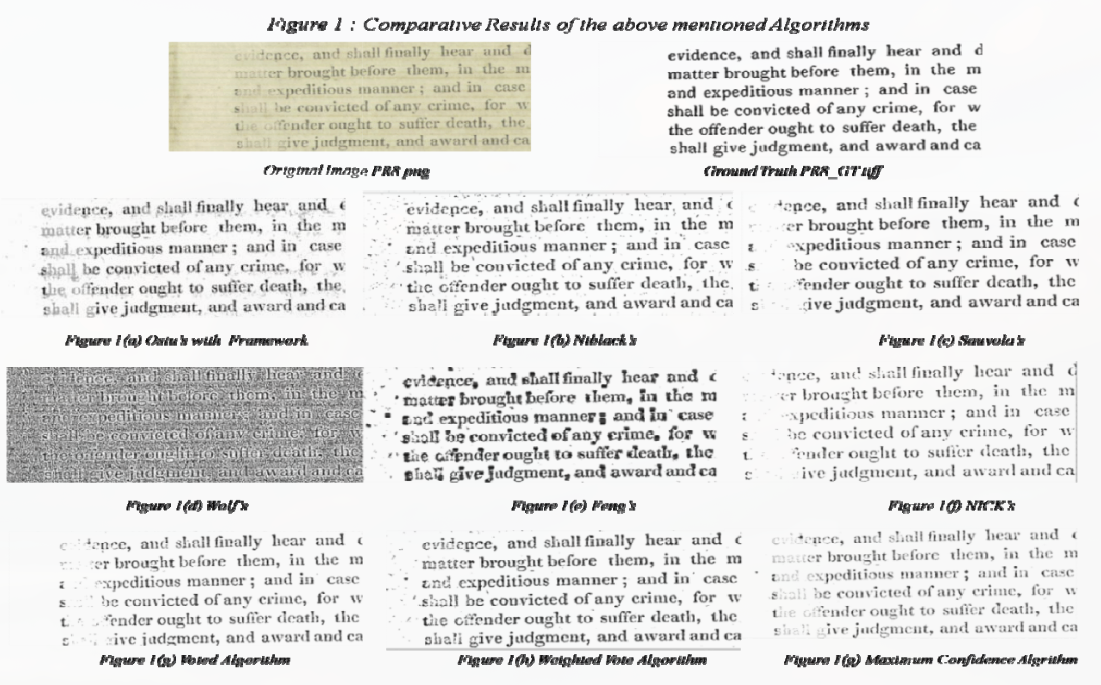
\includegraphics[width=0.9\columnwidth]{figure1.png}
\caption{Comparative Results of the above mentioned Algorithms. (Repeated from Figure 1 for layout.)}
\label{fig:results2}
\end{figure}

\begin{table}[!t]
\caption{COMPARISON OF PROPOSED RESULTS AGAINST WINNING ALGORITHMS OF DIBCO 2011 (continued)}
\centering
\footnotesize
\begin{tabular}{|c|c|c|c|c|}
\hline
\multicolumn{5}{|c|}{PROPOSED METHODOLOGY (VOTED) APPLIED ON 18 RESULTS} \\
\hline
 & VOTED & WT. CONF. & MAX. CONF. & \\
\hline
PR1.png & F-MEASURE & 96.06 & 96.25 & 94.66 \\
 & PSNR & 11.1996 & 11.4083 & 0.8304 \\
\hline
PR2.png & F-MEASURE & 96.11 & 96.35 & 94.91 \\
 & PSNR & 11.2522 & 11.5207 & 0.5714 \\
\hline
PR3.png & F-MEASURE & 97.10 & 97.84 & 97.26 \\
 & PSNR & 12.4848 & 13.7472 & 0.9173 \\
\hline
PR4.png & F-MEASURE & 97.29 & 98.05 & 96.39 \\
 & PSNR & 12.7774 & 14.1731 & 0.5530 \\
\hline
PR5.png & F-MEASURE & 97.57 & 97.71 & 96.35 \\
 & PSNR & 13.2390 & 13.4833 & 0.6765 \\
\hline
PR6.png & F-MEASURE & 90.30 & 89.48 & 85.68 \\
 & PSNR & 7.5230 & 7.2051 & 0.2460 \\
\hline
PR7.png & F-MEASURE & 93.29 & 97.25 & 95.94 \\
 & PSNR & 9.0072 & 12.7070 & 0.1401 \\
\hline
PR8.png & F-MEASURE & 98.15 & 98.16 & 97.69 \\
 & PSNR & 14.3866 & 14.4267 & 0.6767 \\
\hline
AVERAGE & F-MEASURE & 95.74 & 96.39 & 94.86 \\
 & PSNR & 11.48 & 12.33 & 0.5712 \\
\hline
\end{tabular}
\label{tab:voted_on18}
\end{table}

\section*{ACKNOWLEDGMENT}
The authors would like to acknowledge the infrastructural support of the Indian Institute of Information Technology - Allahabad.

\begin{thebibliography}{13}
\bibitem{otsu1979threshold}
N. Otsu, "A threshold selection method from grey level histogram", \textit{IEEE Trans. Syst. Man Cybern.}, vol. 9 no. 1, pp. 62-66 (1979).

\bibitem{chi2012learning}
Z. Chi and K.W. Wong, "A Learning Framework for Degraded Documents Image Binarization using Markov Random Field", \textit{International Conference of Pattern Recognition (ICPR 2012)}, pp.3201-3203, November 2012.

\bibitem{niblack1986introduction}
W. Niblack, "An Introduction to Digital Image Processing", Prentice Hall, Englewood Cliffs, (1986).

\bibitem{sauvola1997adaptive}
J. Sauvola, T. Seppanen, S. Haapakoski, M. Pietikainen, "Adaptive Document Binarization", \textit{4th Int. Conf. On Document Analysis and Recognition}, Ulm, Germany, pp.147-152 (1997).

\bibitem{wolf2003extraction}
C. Wolf, J-M. Jolon, "Extraction and Recognition of Artificial Text in Multimedia Documents", \textit{Pattern Analysis and Applications}, 6(4):309-326, (2003).

\bibitem{feng2004contrast}
Meng-Ling Feng and Yap-Peng Tan, "Contrast adaptive binarization of low quality document images", \textit{IEICE Electron. Express}, Vol. 1, No. 16, pp.501-506, (2004).

\bibitem{khurshid2009comparison}
Khurshid Khurram, Imran Siddiqi, Claudie Faure, and Nicole Vincent. "Comparison of Niblack inspired Binarization methods for ancient documents." In \textit{IS\&T/SPIE Electronic Imaging}, pp. 72470U-72470U. International Society for Optics and Photonics, 2009.

\bibitem{abbyy}
ABBYY Fine Reader Version 12.0, www.finereader.com

\bibitem{dibco2011dataset}
DIBCO-2011 Dataset \\ \url{http://users.iit.demokritos.gr/~bgat/DIBCO2009/benchmark/}

\bibitem{tesseract}
Tesseract OCR - OpenSource, \url{https://code.google.com/p/tesseract-ocr/}

\bibitem{dibco2011results}
DIBCO-2011 Result \\ \url{http://users.iit.demokritos.gr/~kntir/DIBCO13_Results/}

\bibitem{uspatent}
US Patent US6411737B2 \\ \url{https://patentimages.storage.googleapis.com/pdfs/US6411737.pdf}

\bibitem{gatos2011icdar}
B. Gatos, K. Nitrogiannis, and I. Pratikakis, "ICDAR 2011 Document Image Binarization Contest (DIBCO 2011)", \textit{International Conference on Document Analysis and Recognition}, pp.1506-1510, August 2011.
\end{thebibliography}

\end{document}